\documentclass[10pt]{article}
\usepackage{amsmath,amsfonts,amssymb}
\usepackage{mathtools}
\usepackage{color,soul}
\usepackage{fullpage}
\usepackage{enumerate}
\usepackage{graphicx}
\usepackage[colorlinks=true,urlcolor=blue]{hyperref}
\usepackage{subfig}

\definecolor{Light}{gray}{.90}
\sethlcolor{Light}

\title{Fiducial Finding}
\author{Jeren Suzuki}
\date{Last Edited \today}

\begin{document}

\maketitle
\pagenumbering{Roman}
\tableofcontents
\newpage
\pagenumbering{arabic}

\section{Basic Code Overview}
In a nutshell, \hl{\tt{scrib.pro}} takes an image of the sun with fiducials and spits out the positions of the fiducials. How it does this is (in the current iteration of code) it runs two edge-detection filters, isolates pixels above a certain threshold and then calculates what rows/columns the pixels populate most frequently. The result is an array of X and Y positions of the fiducials which we can then orient the sun. 

\section{Outline of Code}
\begin{enumerate}
    \item Load image
    \item Crop image based on known sun center
    \item Apply \hl{\texttt{emboss()}} filter
    \item Apply \hl{\texttt{shift\_diff()}} filter
    \item Create mask based on pixels above threshold
    \item Calculate rows/columns most populated by pixels
    \item Pair the row and column pixels to return fiducial positions
\end{enumerate}

\section{Detailed Code Overview}
    \subsection{Load Image} % (fold)
    \label{sub:load_image}
    I load a .fits file which has no header; alternatively I could load a .tiff directly. However, if I do this, I have to isolate a single channel since I can't save a tiff explicitly as black and white. Even though the image saved has no color, there are still R, G, and B channels which are all identical. The solution is to slice the 3D array into a 2D Array using any of the R, G, or B channels.
    % subsection load_image (end)

    \subsection{Crop image} % (fold)
    \label{sub:crop_image}
    Using values taken from \hl{\texttt{merrygotrace.pro}}, I concentrate on the brightest solar region.
    % subsection crop_image (end)

    % \subsection{\hl{\texttt{emboss}} Filter} % (fold)
    \subsection{emboss Filter}
    \label{sub:emboss_filter}
    The \hl{\texttt{emboss}} filter is a wrapper for IDL's \hl{\texttt{convol()}} function with options to change the convolution kernel. Emboss defaults to look for edges in the x-axis (i.e. left-right direction); you can set an arbitrary ``looking'' angle. Edges in the original image are straddled with high/low values. 

    For example, this is an image of an emboss filter in action:

    \begin{figure}[h]
        \begin{minipage}{0.4\textwidth}
            \begin{center}
            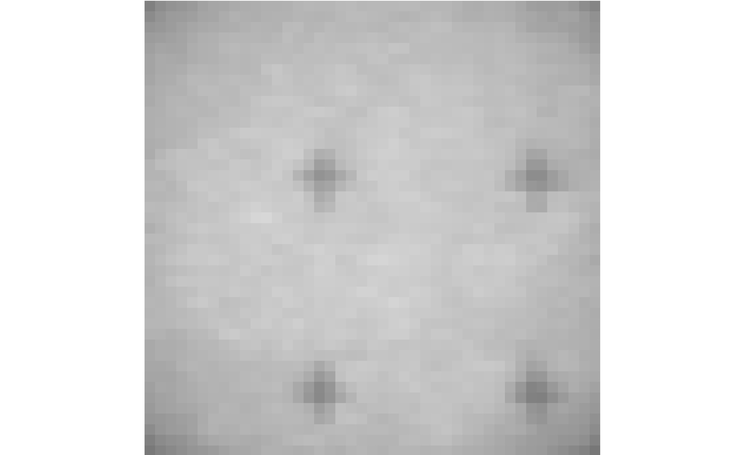
\includegraphics[width=.75\linewidth]{plots_tables_images/untouched.png}
            \caption{Raw image}
            \end{center}
        \end{minipage}
        \begin{minipage}{0.4\textwidth}
            \begin{center}
            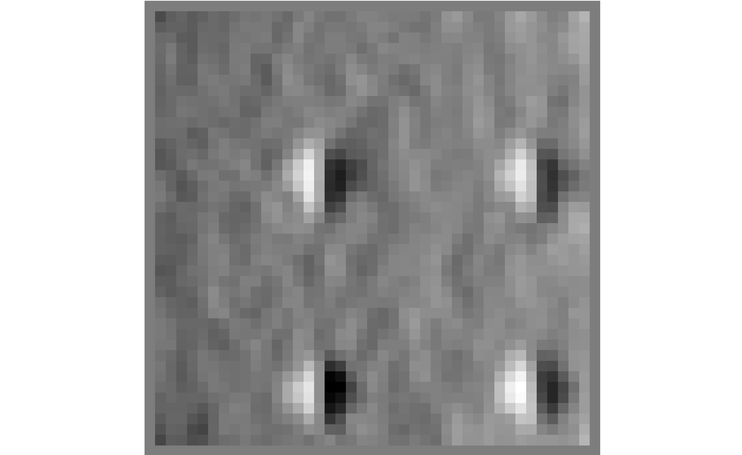
\includegraphics[width=.75\linewidth]{plots_tables_images/emboss.png}
            \caption{Image with \hl{\texttt{emboss()}} filter}
            \end{center}
        \end{minipage}
    \end{figure}
    % subsection emboss_filter (end)

    % \subsection{\hl{\texttt{shift\_diff}} Filter} % (fold)
    \subsection{shift\_diff Filter}
    \label{sub:shift_diff_filter}
    The \hl{\texttt{shift\_diff}} filter takes the \hl{\texttt{emboss}} filtered image and emphasizes the edges created from a large change in a highly negative toa highly positive value (the space between the white and black pixels)

    \begin{figure}[h]
        \begin{minipage}{0.4\textwidth}
            \begin{center}
                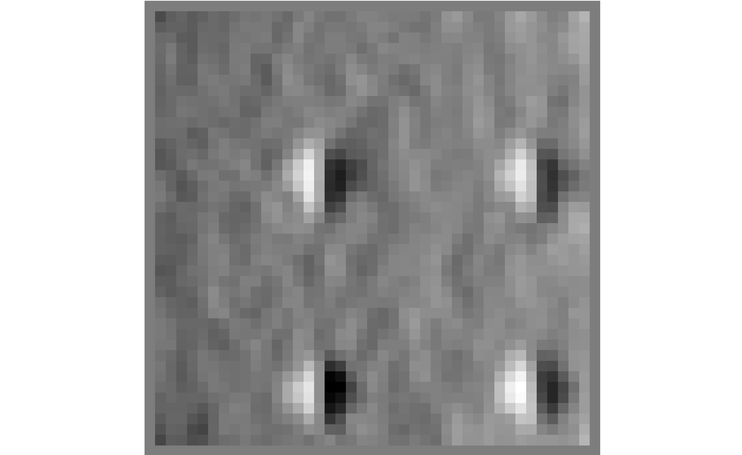
\includegraphics[width=.75\linewidth]{plots_tables_images/emboss.png}
                \caption{Image with \hl{\texttt{emboss()}} filter}
            \end{center}
        \end{minipage}
        \begin{minipage}{0.4\textwidth}
            \begin{center}
                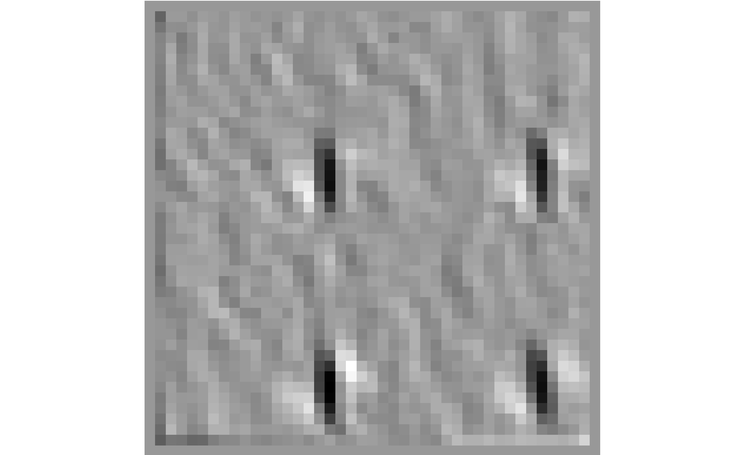
\includegraphics[width=.75\linewidth]{plots_tables_images/shiftdiff.png}
                \caption{Image with \hl{\texttt{emboss()}} filter and \hl{\texttt{shift\_diff()}} filter}
            \end{center}
        \end{minipage}
    \end{figure}
    % subsection \texttt{shift\_diff_filter (end)

    \subsection{Mask Pixels Above Threshold} % (fold)
    \label{sub:mask_pixels_above_threshold}
    Now we have an image with pixels we know are on the fiducials - we look at pixels above a certain threshold to create vertical and horizontal lines which lie on the fiducials. As of \today the threshold is set to an arbitrary value. 

    \begin{figure}[h]
        \begin{minipage}{0.4\textwidth}
            \begin{center}
                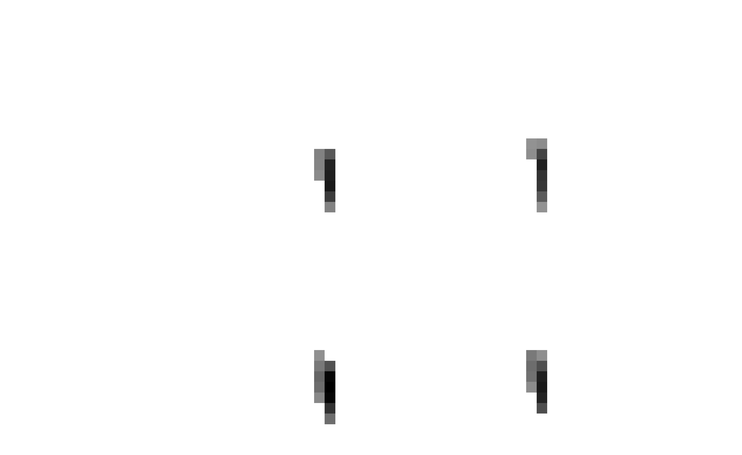
\includegraphics[width=.75\linewidth]{plots_tables_images/below50.png}
                \caption{Pixels below -50}
            \end{center}
        \end{minipage}
        \begin{minipage}{0.4\textwidth}
            \begin{center}
                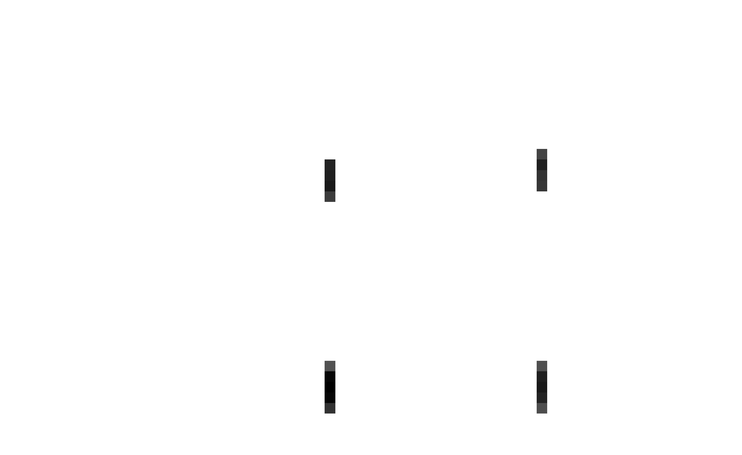
\includegraphics[width=.75\linewidth]{plots_tables_images/below80.png}
                \caption{Pixels below -80}
            \end{center}
        \end{minipage}
    \end{figure}
    % subsection mask_pixels_above_threshold (end)

    \subsection{Calculate Positions of Pixels} % (fold)
    \label{sub:calculate_positions_of_pixels}
    To find the x positions of the pixels I apply a modulo operator to return the remainder of division. (e.g. \hl{\texttt{8 mod 3 = 2}}). To find the y position, I divide the pixel position by the numer of rows. I find the mode of each array of X and Y pixel positions to find the most common number (which happens to be on a fiducial). If there is more than 1 fiducial in the image, the mode must be found for one fiducial then without looking at the same row/column twice, find the second most populated row/column.

    % subsection calculate_positions_of_pixels (end)

\section{Outline of Math}
    \subsection{emboss} % (fold)
    \label{sub:emboss}
    Emboss uses a special kernel:

    \[ \begin{array}{ccc}
    1 &  0 & -1 \\
    1 &  0 & -1 \\
    1 &  0 & -1 \end{array}\] 

     that can be rotated to find edges in a certain direction. For example, \hl{\texttt{emboss(az=90)}} tells the program to look from the 90 degree direction, resulting in a kernel:

     \[ \begin{array}{ccc}
    -1 & -1 & -1 \\
     0 &  0 &  0 \\
     1 &  1 &  1 \end{array}\] 

     The angle can be set to any abitrary value although if the angle is not divisible by 45, the kernel interpolates values between 1 and -1. For \hl{\texttt{emboss(az=30)}}, the kernel looks like:

     \[ \begin{array}{ccc}
    1   & .66   & -.33 \\
    1   &  0    & -1 \\
     .33&  -.66 & -1 \end{array}\] 
    % subsection emboss (end)

    \subsection{shift\_diff} % (fold)
    \label{sub:shift_diff}

    While the kernel can be rotated to any arbitrary angle, we see that rotating the shift\_diff kernel is a bad idea. 

    The shift\_diff kernel looks like

    \[ \begin{array}{ccc}
    0   & 0  & 0 \\
    0   &  1 & -1 \\
    0   &  0 & 0 \end{array}\] 

    Where the center value is always 1 and the position of the -1 index can be changed with keywords. Although the position of -1 can be changed, it can have adverse results on the resulting image. The direction of the ``looking angle'' can be set with a keyword equal to the direction from this matrix:

    \[ \begin{array}{ccc}
    0 & 1 & 2 \\
    3 & x & 4 \\
    5 & 6 & 7 \end{array}\] 

    \begin{figure}[h]
        \begin{minipage}{.45\textwidth}
            % \begin{center}
            \centering
                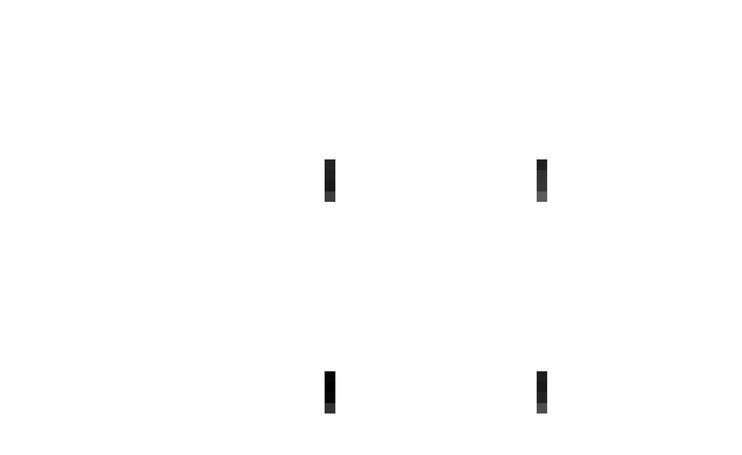
\includegraphics[width=\linewidth]{plots_tables_images/dir3.png}
                \caption{Pixels below -80 and with \hl{\texttt{shift\_diff(dir=3)}}}
            % \end{center}
        \end{minipage}
        \hspace{.5in}
        \begin{minipage}{.45\textwidth}
            % \begin{center}
            \centering
                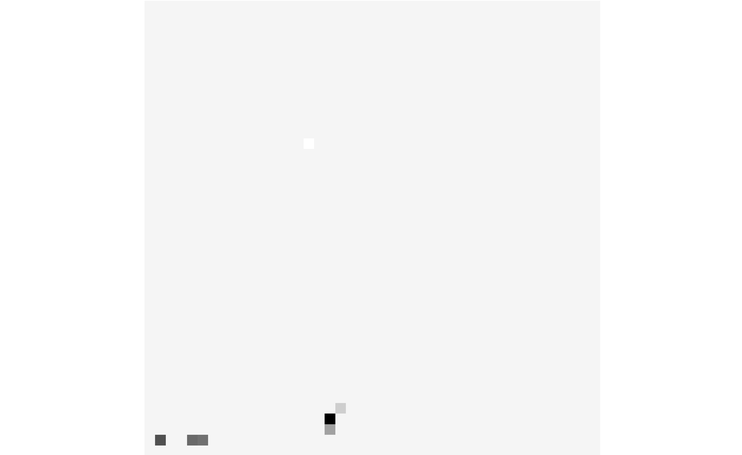
\includegraphics[width=\linewidth]{plots_tables_images/dir1.png}
                \caption{Pixels below -30 and with \hl{\texttt{shift\_diff(dir=1)}}}
            % \end{center}
        \end{minipage}
    \end{figure}

    Basically, if the ``looking angle'' of emboss is perpendicular to the ``looking angle'' of shift\_diff, then the resulting image will have no edges. However, we don't always know how rotated the image is beforehand so it is hard to set the right looking angle. 


    If we expect the fiducials to be rotated only slightly, we can look at the same angle as if the image was not rotated. However, as the angle reaches 90 degrees, we will be increasingly unable to see the fiducials without decreasing the threshold of pixels to mask.

    % subsection shift_diff (end)
\newpage 

\section{More Images}    

\begin{figure}[!ht]
    \centering
    \includegraphics[width=.9\textwidth]{plots_tables_images/fidcomp.eps}    
    \caption{This is a simulated solar image with artificial fiducials. The goal was to see how the filters operated on smudgy fiducials. The results are good. In the second row, the image is filtered with \hl{\texttt{shift\_diff(dir=3)}} and in the third row, the image is filtered with \hl{\texttt{shift\_diff(dir=1)}}. This was done to improve the number of horizontal and vertical pixels for each direction since the default is at a diagonal.}
\end{figure}


\begin{figure}[!ht]
    \centering
    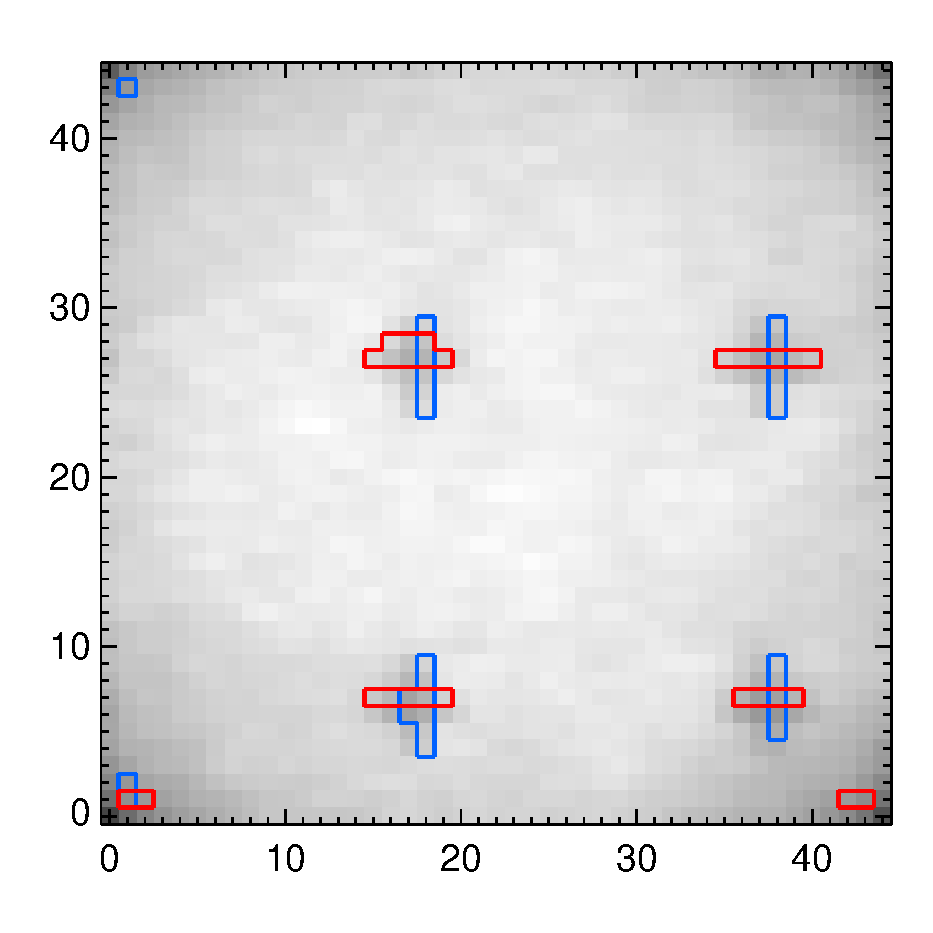
\includegraphics[width=.9\textwidth]{plots_tables_images/mask_outline.eps}
    \caption{The red outline pixels identify those above a threshold after running the two convolution filters. The rows tend to follo a spatial pattern of identifying the upper row of the 2x2 fiducial center. The blue outlined pixels identify the column pixels which are found using a 90 degree offset in the emboss filter. The position where the red and blue outlined pixels overlap mark the upper right pixel of the fiducial's 2x2 center. Since this is consistent for all 4 fiducials, we can confidently apply it to the dimmer suns. \emph{For now}.}
\end{figure}

\begin{figure}[!ht]
    \centering
    \subfloat{
            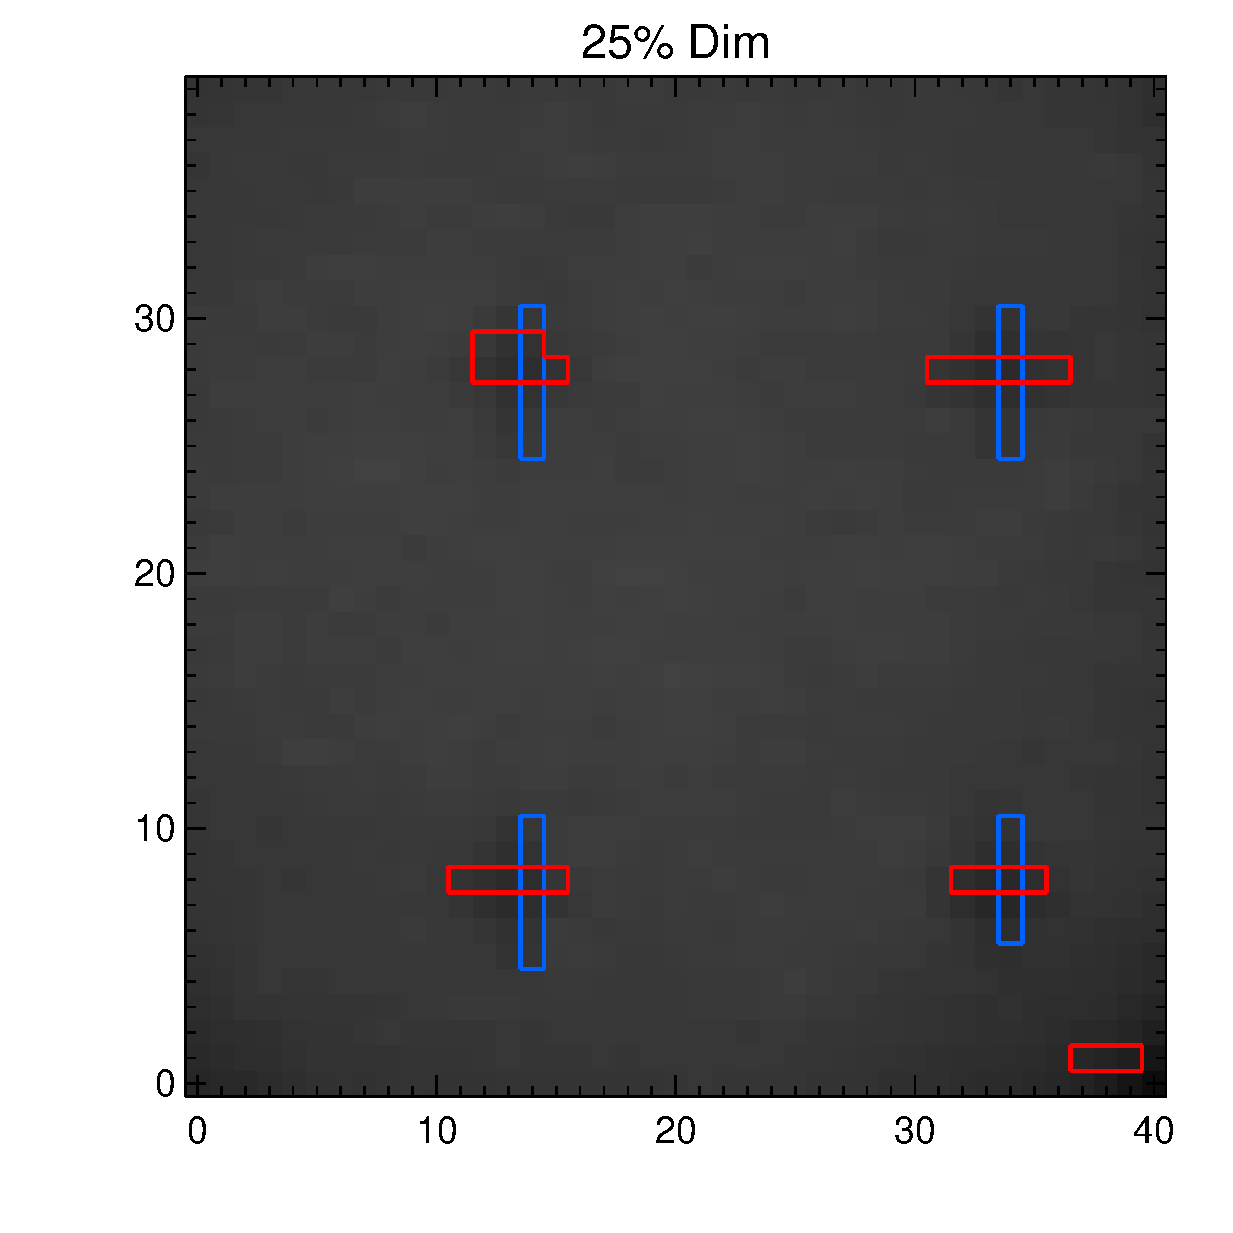
\includegraphics[width=0.98\linewidth, height = .35\textheight, keepaspectratio=true]{plots_tables_images/dim25.eps}
            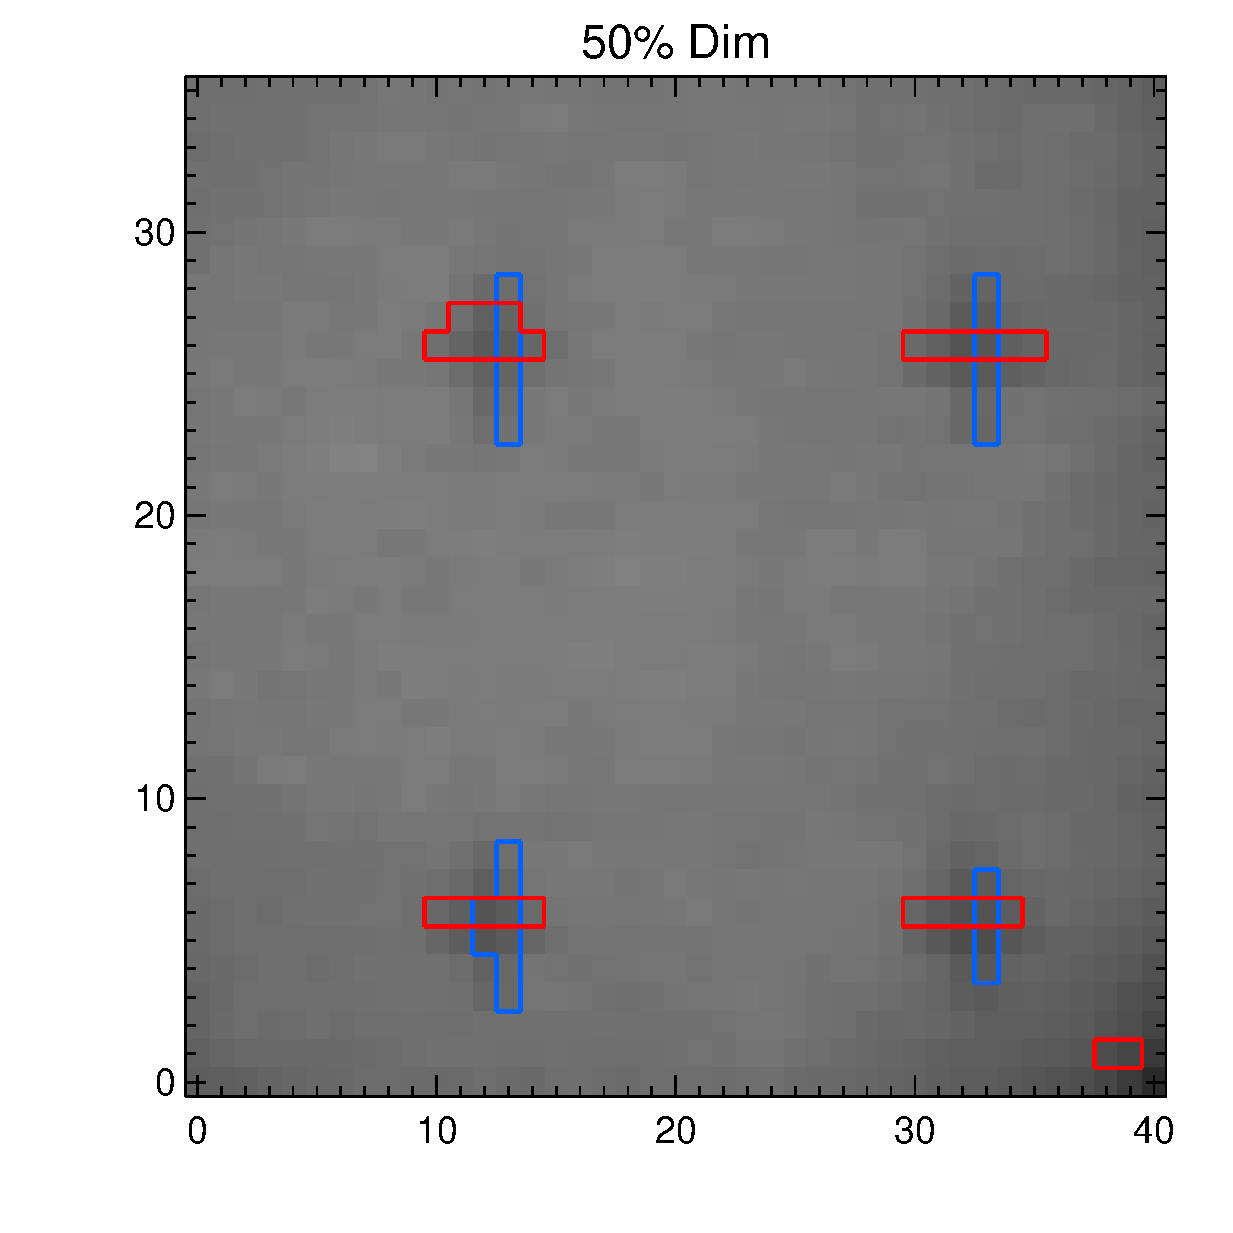
\includegraphics[width=0.98\linewidth, height = .35\textheight, keepaspectratio=true]{plots_tables_images/dim50.eps}
        }
        \caption{By varying the threshold on the dimmer suns, we get the same masking pattern. For the 50\% dimmer sun, we use half the threshold value used for the 100\% sun. For the sun at 25\% the brightness of the main sun, we use a quarter of the threshold.}
\end{figure}


\newpage

\section{Exercises}
    Since our attempt to simulate a realistic fiducial proved lacking quantative reasoning, we looked to extract fiducial values from the real solar image and place them onto a blank (or nearly blacnk, still uniform) 2d array. We found that even if the fiducial pixel values are inconsistent, as long as they form the shape of the fiducial and are substantially different from the the background value, they will appear to be ``perfect''. See Figure \ref{whodunit}

\begin{figure}[!ht]
    \centering
    \subfloat{
            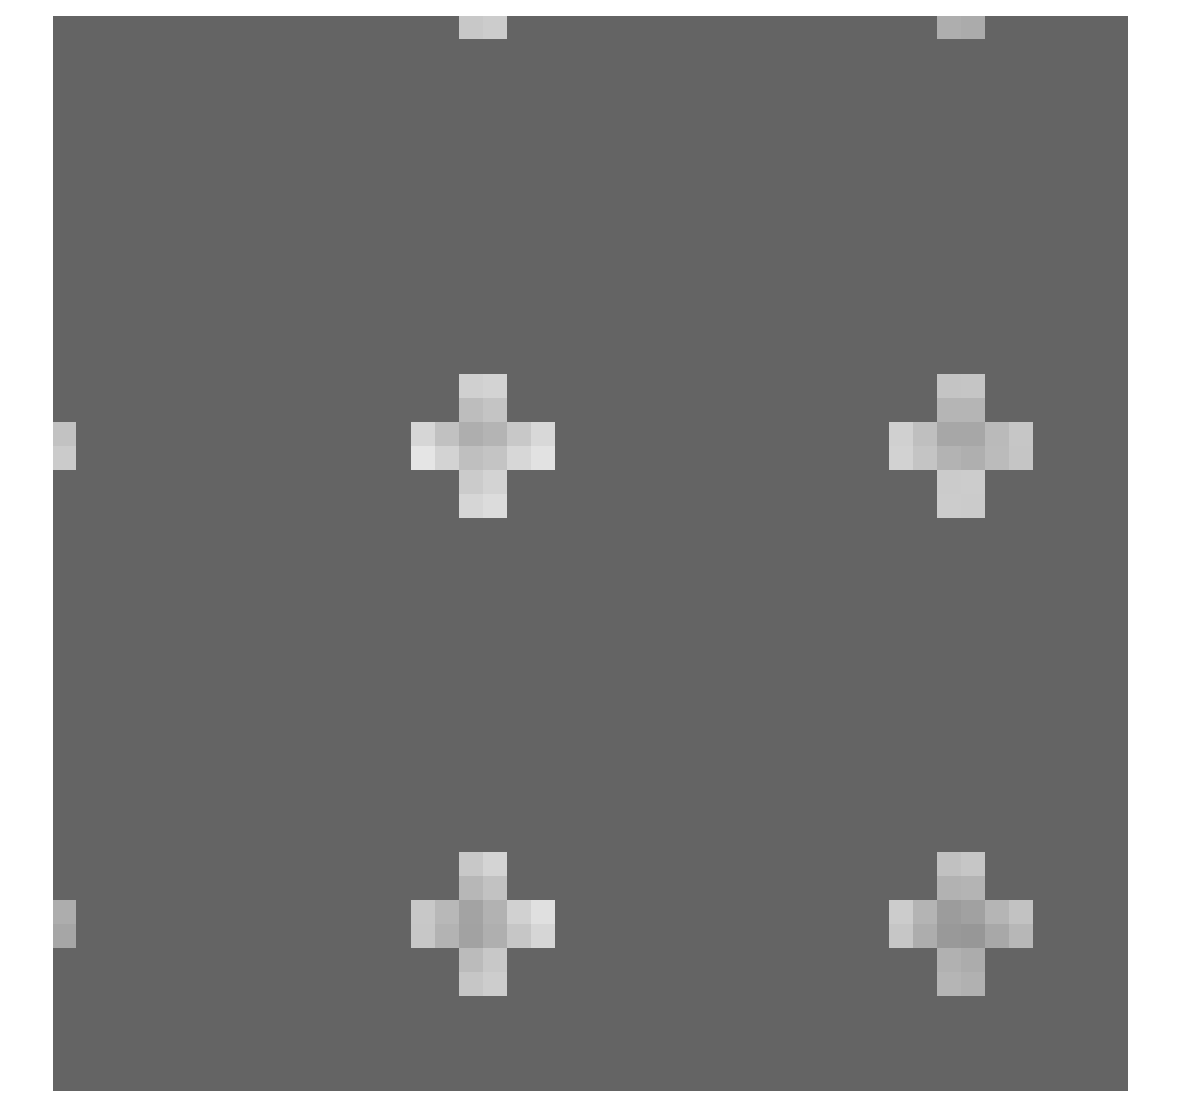
\includegraphics[width=0.98\linewidth, height = .34\textheight, keepaspectratio=true]{plots_tables_images/fakeideal.eps}
            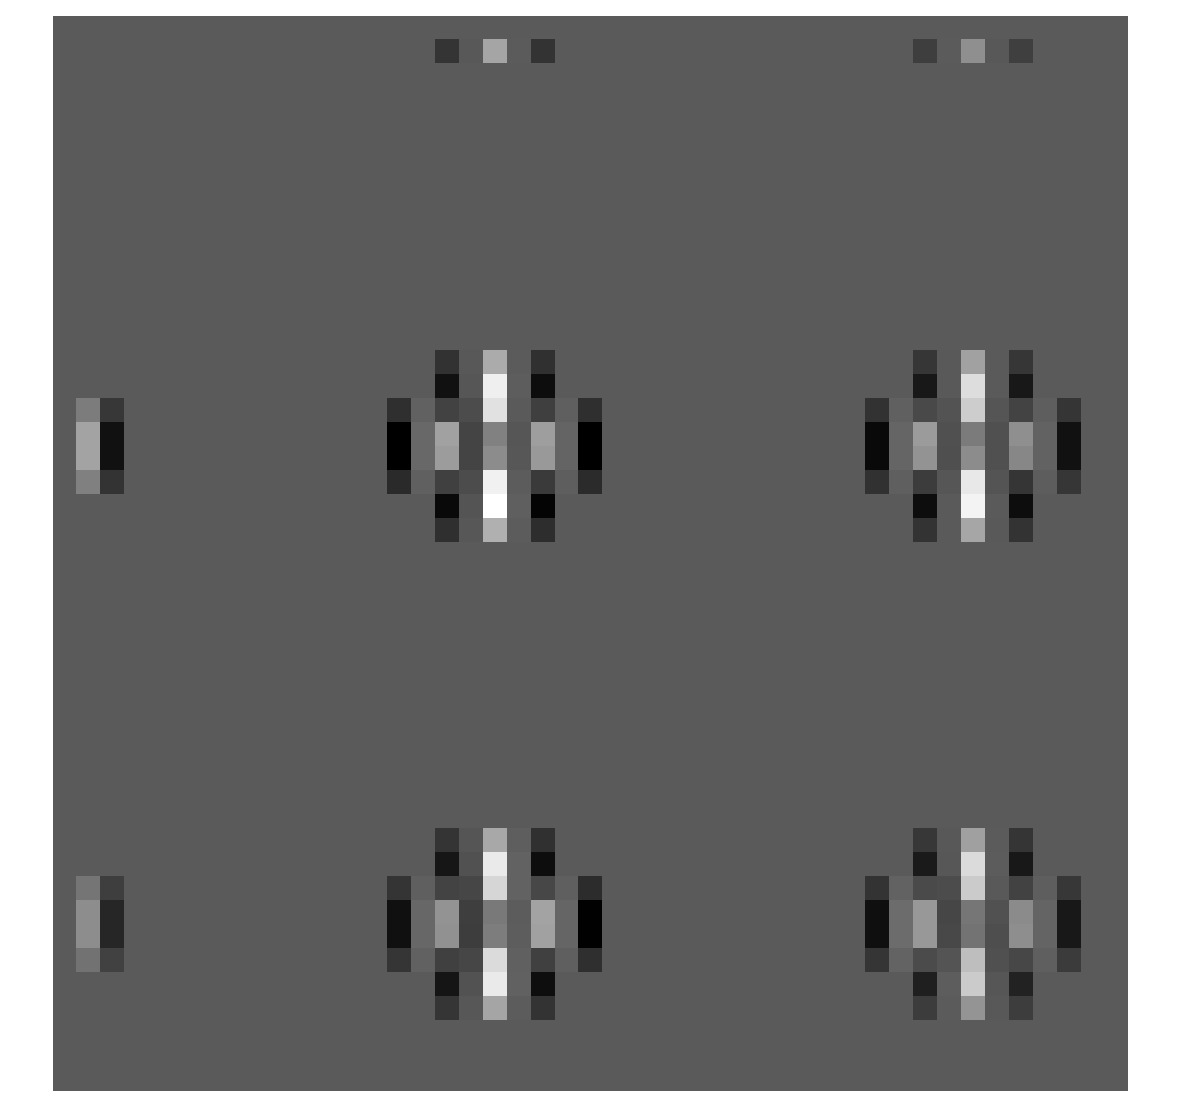
\includegraphics[width=0.98\linewidth, height = .34\textheight, keepaspectratio=true]{plots_tables_images/whodunit.eps}
        }    
        \caption{On the left we see the real fiducial values over a uniform 2D array. On the right is the result of the two convolution filters. Despite the ``blurry'' pixel values, the filters saw the edges of the fiducial.}
    \label{whodunit}
\end{figure}

\begin{figure}[!ht]
    \centering
    \subfloat{
            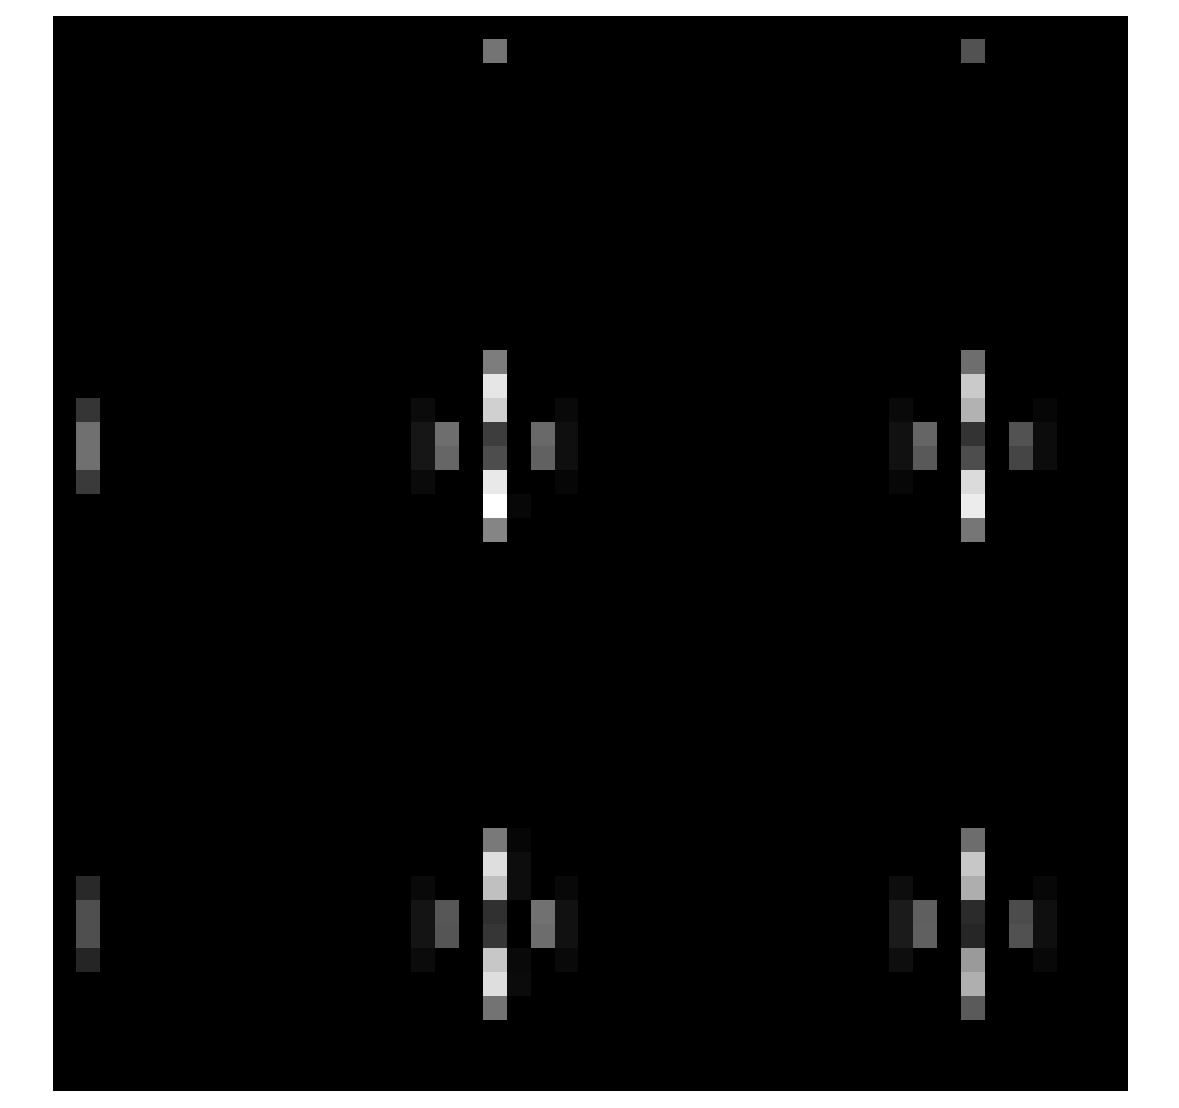
\includegraphics[width=0.98\linewidth, height = .34\textheight, keepaspectratio=true]{plots_tables_images/whodunitwho.eps}
            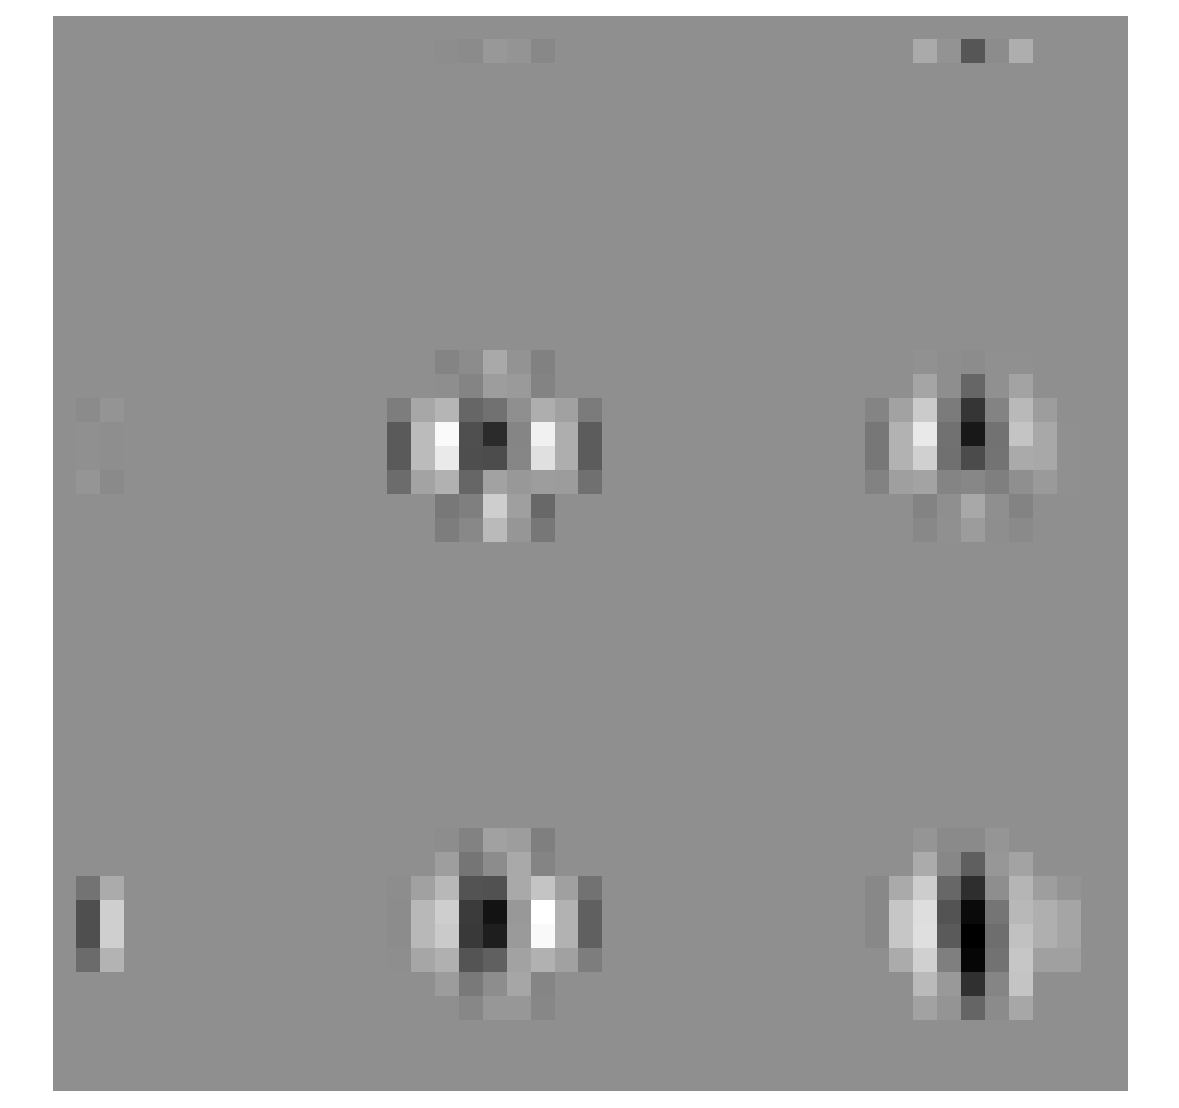
\includegraphics[width=0.98\linewidth, height = .34\textheight, keepaspectratio=true]{plots_tables_images/tryhard.eps}
        }    
        \caption{On the left is the same image as Figure 12(b), but masked to values above a certain threshold. Here you see that there clearly exists a linear structure. I also tried instead of a gray bacground, a background that was equal to the most common pixel value (198 instead of 100). The goal was to try and blur out the fiducial as much as possible. On the right we see the convolution filter has a harder time finding the edges but we still see some clear vertical black lines that we can mask out.}
\end{figure}

\section{Parameters}
    In an effort to keep our work rigorous, attempts have been made to minimize arbitrary variables. These attempts have sometimes failed. Here is a list of parameters to quantize:
    \begin{enumerate}
        \item Width/Height of cropped box of which to look for fiducials in. Must be large enough to cover as much area of the sun as possible witout including the solar limb.
        \item Threshold used to mask twice-convoluted image. As of \today, arbitrary.
        \item ...and others once we recognize them.
    \end{enumerate}

\section{Drawbacks}

    The main problems facing this program are:

    \begin{enumerate}
        \item With rotated fiducials above 2 degrees, cannot use \hl{\texttt{mode()}} to easily find most common pixel positions
        \item With rotated fiducials (and without knowing what angle they are rotated at beforehand), we may have to try multiple rotation angles for the kernels used in each filter.
        \item If the fiducials are not plus-shaped the edge-detection tools cannot handle distortion. Ideally, a circle-shaped fidcial would be fine except that any distortion returns poor results with the edge detection filters. I think this is because the plus-shaped fiducials naturally have up and down edges which, even with distortion, can still be isolated. See Figure \ref{circfidcomp}
        \item We must crop the sun in such a way that none of the solar limb is in the image. The reason is because the image is pixelated enough that the edge of the sun is detected as an edge, albeit one we do not want. A problem that arises from this is that when we crop out the solar limbs, we may cut off fiducials.
        \item If the fiducial is too close to the edge of the cropped image, then problems arise. There are two ways to solve this. We can tell the program to only look for complete fiducials or 2) ``zero'' out the incomplete fiducials so the program finds fiducials as normal.
        \item In \hl{\texttt{circscancrop}}, the thresholds are arbitrary. To scan for region 2, (i.e., the 50\% brightness sun) we have the threshold set to 0.3 of the sorted \hl{\texttt{max(image)}}. For region 3 (i.e., the 25\% brightness sun) the threshold is set to 0.2 of the sorted \hl{\texttt{max(image)}}. I tried making the threshold 0.3 of the image with the highest 1\% pixels eliminated, but the change in threshold made the circle-scanning break. Either I need to find a new way to parameterize the thresh or change the circle-scanning code. 
        \item The fiducial positions for the 25\% sun seem to be wrong. This is either because of a wrong center position or the fiducial finding code not working properly (inclined to agree with first result, 100\% and 50\% brightness suns look identical, must be something wrong with the 25\% brightness sun. Right?)
    \end{enumerate}

\begin{figure}
    \centering
    \includegraphics[width=.9\textwidth]{plots_tables_images/circfidcomp.eps}
    \caption{The fiducials are initially circles but with a bit of distortion we see the typical method to find fiducials no longer works. Perhaps with circle-shaped fiducials we could apply some form of gaussian fitting but using plus-signs instead works better since it's hard to calculate the rotation angle from a bunch of distorted circles.}
    \label{circfidcomp}
\end{figure}


\section{How to Break Code} % (fold)
\label{sec:how_to_break_code}

    \begin{enumerate}
        \item Sun is too close to the edge of the solar image\\
            - When cropping, either need to fabricate null data or ignore altogether
        \item Part of sun is cut off in image\\
            - Not only will cropping fail, limb fitting will also fail
        \item Bad pixels\\
            - Threshold finding has been changed to remedy this
        \item When scanning in a circle, haven't completely coded fail-safes if it doesn't find auxilliary suns\\
            - Probably have to do something where if I don't detect the auxilliary suns, I'll scan at different readii at specific intervals
        \item Image is rotated more than 2 degrees\\
            - Current fiducial finding method can't handle a rotated image well
            - GRIPS proposal says the pendulum will swing up to $\pm$ .1 degree; is this the same rotation parameter in our image?
        \item Fiducial is too close to edge\\
            - If a fiducial is too close to edge of cropped image, incomplete fiducial shape confuses program
            - Not sure how to fix yet (\today)
    \end{enumerate}

% section how_to_break_code (end)

\end{document}